%\documentclass[openright,twoside,headsepline]{scrbook}
%\usepackage[applemac]{inputenc}
%\usepackage{graphicx,xcolor,hyperref} % obsolete in HU-diss
%\usepackage[round,authoryear]{natbib}
%\setlength\bibhang{2em} 
%
%
%\KOMAoptions{numbers=noenddot}
\usepackage{amsmath,amssymb,amsfonts,amsthm,epigraph,scrpage2}
\usepackage[ngerman,english]{babel}
\definecolor{Cayenne}{rgb}{0.502,0.0,0.0}
\definecolor{Steel}{rgb}{0.4,0.4,0.4}


%\setcounter{secnumdepth}{3} % sub subsections numbering
%\setcounter{tocdepth}{3} % subsubsections inTOC

\usepackage[format=plain,singlelinecheck=false, font={sf,small},labelfont={bf,color=Steel}]{caption}
\DeclareCaptionLabelSeparator{cayenne_period}{\textcolor{Cayenne}{.} }
\captionsetup{labelsep=cayenne_period}

% Colors
\addtokomafont{chapter}{\color{Steel}}
\addtokomafont{section}{\color{Steel}}
\addtokomafont{subsection}{\color{Steel}}
\addtokomafont{subsubsection}{\color{Steel}}
\addtokomafont{paragraph}{\color{Steel}}

\addtokomafont{pagehead}{\color{Steel}}
\renewcommand{\pnumfont}{\color{Steel}} 
\addtokomafont{headsepline}{\color{Steel}} 
\pagestyle{scrheadings} 

%\makeatletter % dot after sections and all below
%\let\std@sect\@sect
%\def\@sect#1#2#3#4#5#6[#7]#8{\std@sect{#1}{#2}{#3}{#4}{#5}{#6}[#7.]{#8\color{Cayenne}{.}}}
%\makeatother

\usepackage[leftcaption]{sidecap} % inner, outer,left,right
\sidecaptionvpos{figure}{t}

% Papiergr��e
%\setlength{\paperwidth}{24cm}
%\setlength{\paperheight}{17cm}
%\recalctypearea
%\usepackage{geometry}

%% Flattersatz
%\usepackage[document]{ragged2e} % Flattersatz
%\setlength{\RaggedRightParindent}{1em} % evtl. parskip


%% Sans Serif
%\usepackage{cmbright}
%\renewcommand{\familydefault}{\sfdefault}
%% Palatino
%\usepackage[sc]{mathpazo}
%\linespread{1.05}         % Palatino needs more leading (space between lines)
%\setkomafont{sectioning}{\normalcolor\bfseries} % Kapitel�berschriften

%%% Kapitel�berschriften: Mit gro�en Zahlen
%\usepackage{titlesec}
%\titleformat{\chapter}[display]
%{\bfseries\Large}
%{ %\Huge\textsc{\chaptertitlename} % f�r das Wort 'Kapitel'
%\hfill\fontsize{120}{70}\selectfont\color{lightgray}\textbf{\thechapter}}
%{-2ex}
%%{\filleft\fontsize{50}{70}\selectfont\scshape} % Kapit�lchen oder...
%{\filleft\fontsize{50}{70}\selectfont\textbf} % ...oder keine Kapit�lchen
%[\vspace{0ex}]
%
%%%% Part�berschriften
%\titleformat{\part}[display]
%{\bfseries\Large}
%{ %\Huge\textsc{\chaptertitlename} % f�r das Wort 'Kapitel'
%\hfill\fontsize{120}{70}\selectfont\color{lightgray}\textbf{\thepart}}
%{-2ex}
%{\filleft\fontsize{50}{70}\selectfont\scshape} % Kapit�lchen oder...
%%{\filleft\fontsize{50}{70}\selectfont\textbf} % ...oder keine Kapit�lchen
%[\vspace{0ex}]


\newcommand{\ER}{Erd\H{o}s-R\'enyi }
\newcommand{\BA}{Barab\'asi-Albert }
\newcommand{\mean}[1]{\left< #1 \right>}
\newcommand{\abs}[1]{\left| #1 \right|}
\newcommand{\norm}[1]{\lVert#1\rVert}
\newcommand{\mat}[1]{\mathbf{#1}}
\newcommand{\tgraph}{\mathcal{G}}

\theoremstyle{definition} % non-italic
\newtheorem{annahme}{Annahme} % braucht amsthm
\newtheorem{definition}{Definition}
\newtheorem{theorem}{Theorem}
\newtheorem{satz}{Satz}
\newtheorem{frage}{Frage}
%\input{watermarks/watermark.tex}
\DeclareMathOperator{\nnz}{nnz}

% + Graphicspath nach begin document

%
%
%
%\begin{document}
%\graphicspath{{/Users/lentz/Documents/GitHub_locals/Thesis/images/}}
%\tableofcontents
%


\chapter{Static livestock trade network}
In this chapter, we address the analysis of static networks, where the focus lies on epidemic spread on networks.
Large amounts of data about different contact structures between a huge amount of subjects became available in the last years.
In the context of epidemics, different types of networks can be obtained.
Concerning infectious diseases of humans, it is unlikely to have the exact contact data of a (sub)-population.
Different methods to extract the contacts structure can be used \citep{Keeling:2005}:
\emph{Contact tracing} is used to determine infection paths under the assumption that every contact has a high probability to cause an infection.
This assumption is justified for highly contagious diseases, such as influenza or sexually transmitted diseases \citep{Rocha_pnas,Rocha_plosbc}.
If more data is available, one can obtain an \emph{infection tracing} network, where every contact definitely caused an infection.
Infection tracing plays an important role for the analysis of HIV spread or food safety \citep{Wilking,Haydon22012003}.
\emph{Diary-based} methods make use of questionnaires to extract contact structures.
The drawback of this method is that the subjects themselves are responsible for the information given and a considerable bias can be present in the data \citep{Visser:2003p784}.
Other diary-based methods make use of legislation in order to guarantee for a sufficient data quality.
An example is the HI-Tier database, which records trade movements of livestock animals and is used for food safety and is a central subject of study in this work \citep{Euro-Lex}.

Based on the amount of available data as quoted above, it is reasonable to model epidemics using a purely topological analysis.
Detailed epidemiology is by far more complex as solving differential equations.
Fine-grained models including large sets of parameters and couplings are needed to model infectious diseases.
A complex example for the transmission of classical swine fever is found in \citep{MartinezLopez:2011db}.
In general, a detailed knowledge about infection probability, contact probability and sensitivity to initial conditions is required to obtain a realistic epidemic model.
Even if this information was available, results could not necessarily be generalized to other systems.

For this reason we restrict the epidemiological aspect of this work to a purely topological analysis of the underlying networks, where detailed data about contact structures is available.
In particular, we focus on a network of pig trade in Germany in the years 2009--2010.
Each node in this network represents an agricultural holding and trade contacts between holdings are represented by directed edges.
This chapter is devoted to a static network analysis of this system and a general topological classification.
In section XX we highlight the effects of a time-resolved treatment of these systems.

\paragraph{Livestock trade dataset\color{Cayenne}{.}}
After the BSE crisis in Europe in 2001, the EU member states established livestock trade movement databases to track potential pathways of pathogen spread.
Since 2001, every holding in Germany is obliged to report every trade movement of live animals (pig, cattle, sheep and goat) to a federal database (\foreignlanguage{ngerman}{Herkunftssicherungs und Informationssystem f�r Tiere} (HIT), \citep{HI-Tier}).
We focus on the trade contacts for pigs.
Trade is recorded in a temporal resolution of 1 day, where the receiving holding and the pre-owner are reported in the database.
In this section we aggregate the trade contacts yielding a static network, where a trade edge is present, if there was at leaf one trading contact during the observation period.
Our data extract spans the trade within Germany between january 2009 and march 2010.



\section{Network analysis}
To begin with, we analyze the livestock trade data according to the measures introduced in section \ref{sec:network_measures}.
\paragraph{Centrality and distances\color{Cayenne}{.}}
Figure \ref{fig:hit_deg_cdf} shows the heavy-tailed degree distribution of the network.
%
\begin{SCfigure}
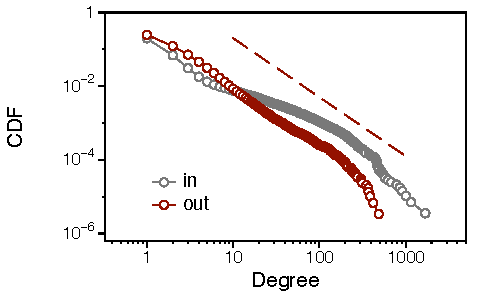
\includegraphics{HIT_Degree_CDF.pdf}
\caption{Degree distribution of the livestock trade network. The out-degree distribution (red) is well approximated by a power-law of the form $x^{-1.6}$ (red dashed line).
The in-degree distribution shows a bimodal behavior indicating large slaughterhouses.
}
\label{fig:hit_deg_cdf}
\end{SCfigure}
%

\paragraph{Components and ranges\color{Cayenne}{.}}
Ignoring the edge direction, the network has a giant component containing more than 98~\% of the nodes. The second largest weakly connected component contains only 11 nodes.
The size of the largest and second largest strongly connected components are 21,8~\% and  0.05~\% (47 nodes), respectively.
Sizes of the next smaller components decrease rapidly.
All in all the network percolates ignoring the direction of links.
Taking into account link directions, the giant component contains a considerable fraction of the network, but is far from the percolation threshold.

The giant strongly connected component has an interesting impact on the distribution of node ranges (and reachabilities) in the network.
Node that the range of a node defines the upper bound for any disease outbreak starting from this very node.
\begin{figure}[htbp]
\begin{center}
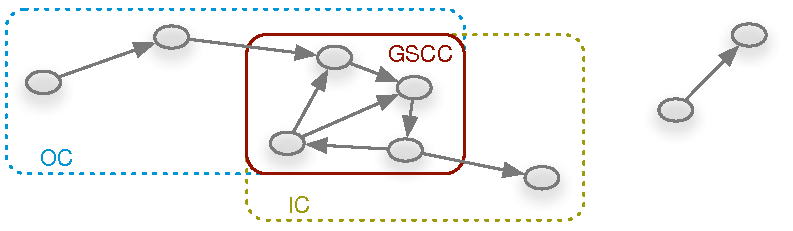
\includegraphics{RangeGap-principle.pdf}
\caption{Schematic structure of a directed network.
In the core region there is the giant strongly connected component (GSCC, red). All nodes reachable from the GSCC form the in-component of the network (IC, yellow) and the nodes with access to the GSCC define the network out-component (OC, blue).
The two nodes on the right are not (weakly) connected to the giant component.
}
\label{fig:rangegap_principle}
\end{center}
\end{figure}



%
%\bibliographystyle{apalike}
%\bibliography{/Users/lentz/Documents/GitHub_locals/Thesis/bibliography.bib}
%\end{document}

